\documentclass[10pt]{article}
\usepackage{titlesec}
\usepackage{titling}
\usepackage[margin=0.8in]{geometry}
\usepackage{graphicx}
\usepackage{hyperref}
\usepackage[export]{adjustbox}


\titleformat{\section}
{\large }
{}
{0.0em}
{\bfseries \uppercase}

\titleformat{\subsubsection}[runin]
{\large \bfseries \uppercase}
{}
{0em}
{}

\titlespacing{\subsubsection}
{0em}{0em}{0em}

\renewcommand{\maketitle}{
	\begin{center}
	{\bfseries \Huge
	\theauthor}
	\rule{17.5cm}{1pt}
	\end{center}	
}

\begin{document}

	% Name
	\author{Prakash Sanyasi}
	\maketitle
	
	% ,Address,Contact information (Contact,e-mail), Photograph 
	\begin{minipage}{0.5\linewidth}
		\href{http://cst.edu.bt/}{\bf College of Science and Technology} \\
		{\bf Rinchending : Phuntsholing} \\
		{\bf Chhukha : Bhutan}\\ \\
		{\bf Contact: } (+975) 17965898 \\
		{\bf Email: } \href{mailto:prakashsanyasi619@gmail.com}{\tt prakashsanyasi619@gmail.com} \\
	\end{minipage}
	\begin{minipage}{0.45\linewidth}
		\raggedleft
		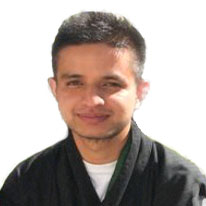
\includegraphics[width=0.4\textwidth]{cover_photo}
	\end{minipage}

 
\end{document}